


\begin{document}

\noindent This proposal is written in reply to a call for proposals for novel applications of the transmitter module of the Optical Uplink project. The overall block diagram of the Optical Uplink can be seen in Figure \ref{fig:blockdiagram2}.


\begin{figure}[H]
    \centering
    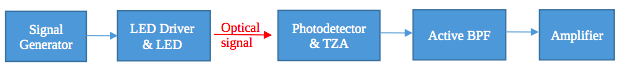
\includegraphics[width=.9\textwidth ]{Introduction/blockdiagram}
    \caption{Block diagram for optical uplink}
    \label{fig:blockdiagram2}
\end{figure}

The Optical Uplink project was finalized with the implementation of an LED signal transmitter with a separate receiver/amplifier module. The entire device acts as a rudimentary wireless communication device capable of transmission over tens of meters.

An infrared sensor, widely known as a tripwire, is a popular device that has many applications, notably in both military and retail. In this proposal, the use of IR as trigger method for IR will be considered, and the importance of tripwire sensors in retail will be discussed.


%%Actual proposal stuff goes here



\end{document}